\documentclass[11pt,a4paper]{article}
\usepackage[margin=2.2cm]{geometry}
\usepackage{fontspec}
\setmainfont{TeX Gyre Pagella}
\setmonofont{DejaVu Sans Mono}[Scale=0.82]
\usepackage{amsmath,amssymb,amsthm}
\usepackage{graphicx,xcolor,listings,booktabs,enumitem}
\usepackage[most]{tcolorbox}
\usepackage{tikz}
\usepackage{needspace}
\usepackage[hidelinks]{hyperref}

\definecolor{accent}{HTML}{2B6CB0}
\definecolor{warn}{HTML}{C53030}
\newtcolorbox{keybox}[1][]{colback=accent!5,colframe=accent,boxrule=0.6pt,arc=2pt,left=6pt,right=6pt,top=4pt,bottom=4pt,#1}
\newtcolorbox{warnbox}{colback=warn!5,colframe=warn,boxrule=0.6pt,arc=2pt,left=6pt,right=6pt}

\lstdefinelanguage{Rust}{
  keywords={fn,let,mut,if,else,for,in,while,return,use,pub,struct,impl,loop,break,Some,None,as,match,const,Self,self},
  morekeywords=[2]{usize,i32,i64,u64,f64,bool,Vec,VecDeque,BTreeSet,BTreeMap,BinaryHeap,Option,str},
  sensitive=true, morecomment=[l]{//}, morestring=[b]"}
\lstset{language=Rust,basicstyle=\ttfamily,keywordstyle=\color{accent}\bfseries,
  keywordstyle=[2]\color{teal},commentstyle=\color{gray}\itshape,stringstyle=\color{warn},
  frame=single,rulecolor=\color{gray!40},backgroundcolor=\color{gray!4},
  numbers=left,numberstyle=\tiny\color{gray},xleftmargin=1.5em,breaklines=true,
  columns=fullflexible,keepspaces=true,showstringspaces=false}

\newtheorem*{invariant}{Invariant}
\theoremstyle{definition}\newtheorem*{definition}{Definition}

\usepackage{soul}
\definecolor{hlY}{HTML}{FFF3A0}\definecolor{hlG}{HTML}{C8F2C2}\definecolor{hlP}{HTML}{E6D2F7}\definecolor{hlB}{HTML}{CFE3FF}
\newcommand{\hly}[1]{{\sethlcolor{hlY}\hl{#1}}}
\newcommand{\hlg}[1]{{\sethlcolor{hlG}\hl{#1}}}
\newcommand{\hlp}[1]{{\sethlcolor{hlP}\hl{#1}}}
\newcommand{\hlb}[1]{{\sethlcolor{hlB}\hl{#1}}}
\newcommand{\img}[3]{\begin{center}\fcolorbox{gray!50}{white}{\includegraphics[width=#1]{board/#2}}\\[-2pt]{\footnotesize\textcolor{gray}{#3}}\end{center}}
\newcommand{\extra}{\textsuperscript{\textcolor{warn}{[extra]}}}
% pages of the prof's 2025 notes on the Fenwick tree (Lessons/L11/FenwickTree_2025.pdf)
\newcommand{\oldnotes}[2]{\begin{center}\fcolorbox{gray!50}{white}{\includegraphics[page=#1,width=#2,trim=20 20 20 20,clip]{../L11/FenwickTree_2025.pdf}}\\[-2pt]
  {\footnotesize\textcolor{gray}{Prof.'s notes of \textbf{last year} (2025), \texttt{FenwickTree\_2025.pdf} p.\,#1}}\end{center}}
\newcommand{\twonotes}[2]{\begin{center}\begin{minipage}{0.49\textwidth}\centering\fcolorbox{gray!50}{white}{\includegraphics[page=#1,width=0.95\linewidth,trim=20 20 20 20,clip]{../L11/FenwickTree_2025.pdf}}\end{minipage}\hfill
  \begin{minipage}{0.49\textwidth}\centering\fcolorbox{gray!50}{white}{\includegraphics[page=#2,width=0.95\linewidth,trim=20 20 20 20,clip]{../L11/FenwickTree_2025.pdf}}\end{minipage}\\[2pt]
  {\footnotesize\textcolor{gray}{Prof.'s notes of \textbf{last year} (2025), \texttt{FenwickTree\_2025.pdf} p.\,#1 and p.\,#2}}\end{center}}
\newcommand{\board}[3]{\img{#1}{#2}{Board, #3 (recording \texttt{L\_13.MP4})}}
\newcommand{\stnotes}[2]{\begin{center}\begin{minipage}{0.49\textwidth}\centering\fcolorbox{gray!50}{white}{\includegraphics[page=#1,width=0.95\linewidth,trim=20 20 20 20,clip]{Segment_tree_2025.pdf}}\end{minipage}\hfill
  \begin{minipage}{0.49\textwidth}\centering\fcolorbox{gray!50}{white}{\includegraphics[page=#2,width=0.95\linewidth,trim=20 20 20 20,clip]{Segment_tree_2025.pdf}}\end{minipage}\\[2pt]
  {\footnotesize\textcolor{gray}{Prof.'s notes of \textbf{last year} (2025), \texttt{Segment\_tree\_2025.pdf} p.\,#1 and p.\,#2}}\end{center}}
\title{\textbf{CPC --- Lecture 13}\\[2pt]\large Update the Array $\cdot$ Range updates with two Fenwick trees $\cdot$ Segment tree (introduction)}
\author{Competitive Programming and Contests --- Wednesday 28/10/2026}
\date{}

\begin{document}\sloppy
\maketitle
\vspace{-1.5em}
\begin{keybox}
\textbf{Sources.} Recording \texttt{Lessons/L13/L\_13.MP4} (97 min; \hlp{it starts a few seconds into the statement of the first problem}) and its automatic transcript
\texttt{L13\_transcript.txt} (not revised); the prof's handwritten board (frames of the recording, \texttt{board/l13\_*.jpg});
the prof's 2025 notes \texttt{Lessons/L11/FenwickTree\_2025.pdf} (p.\,11--15) and \texttt{Lessons/L13/Segment\_tree\_2025.pdf} (p.\,1--2);
the prof's blog post \emph{Dynamic Prefix Sums with Fenwick Tree} (\url{https://pages.di.unipi.it/rossano/blog/2023/fenwick}), code copied verbatim.
No notes of yours for this lecture. Everything marked \extra{} was \emph{not} said or written in the lecture.

\smallskip
\noindent Code: \texttt{Lessons/L13/src} (\texttt{cargo test -p l13}). Exercises: \texttt{Lessons/L13/practice}, E53--E55 (\texttt{cargo test -p practice\_l13}).

\smallskip
\noindent\textbf{Highlights:} \hly{general / to remember} \quad \hlg{good: works, efficient, correct} \quad \hlp{bad: pitfalls, wrong ideas, costs} \quad \hlb{definitions and key results}
\end{keybox}

\begin{keybox}[colback=gray!4,colframe=gray!60]
\textbf{Where we are.} L12 (26/10) did counting inversions with the Fenwick tree, remapping, Nested Segments, and the prof announced ``another lecture about this kind of stuff''.
Today: the two problems left from the 21/10 row of the course page, \textbf{Update the Array} (0:00--16:00) and \textbf{dynamic prefix sums with range update} (16:00--66:00, with a digression on ETH),
then the \textbf{segment tree} (66:00--97:00). These two problems were in the Appendix of the provisional L12; now they are here.
\end{keybox}

\tableofcontents

%==========================================================
\section{Update the Array (SPOJ UPDATEIT)}
%==========================================================
\textbf{Problem.} Given $A[1,n]$, initially $A[i]=0$ for all $i$, support
\hlb{\mbox{$\textsf{Access}(i)=A[i]$}} and \hlb{\mbox{$\textsf{Update}(i,j,v)$}: \mbox{$A[k]\mathrel{+}=v$} for all \mbox{$k\in[i,j]$}}.
Example on the board: $\textsf{Update}(2,6,10)$, $\textsf{Update}(0,4,5)$, $\textsf{Access}(2)=15$.
\board{0.55\textwidth}{l13_update_statement.jpg}{9:00}
\textbf{Trivial solution}: store $A$ and update by scanning: \hlg{\textsf{Access} \mbox{$O(1)$}}, \hlp{\textsf{Update} \mbox{$\Theta(j-i+1)$}: terribly slow for large ranges}.
Target: \hlb{both in \mbox{$\Theta(\log n)$}}.

\noindent\textbf{Wrong directions from the class.}
\begin{itemize}[nosep]
\item Store the prefix sums $P$ of $A$ (5, 20, 35, 50, 60, 70, 70, \dots) and access by difference of consecutive values.
\item Store $A$ itself in a Fenwick tree and update every position of the range: \hlp{\mbox{$\Theta((j-i+1)\log n)$}, worse than the trivial solution}.
      ``Your intuition was right, but you were doing the opposite: you were storing $A$ to get the prefix sums.''
\end{itemize}
\textbf{Idea} (a student, 10:00): \hlb{store \mbox{$V[1,n]$} such that \mbox{$A[i]=\sum_{k\le i}V[k]$}}. \hly{The same trick as the \mbox{$+1/-1$} of Little Girl (L10)}:
a value added at a position propagates to the right through the prefix sums, and $-v$ after the range cancels the propagation.
\begin{itemize}[nosep]
\item $\textsf{Update}(2,6,10)$: $V[2]\mathrel{+}=10$, $V[7]\mathrel{-}=10$: the prefix sums give $10$ on positions $2..6$ and $0$ after.
\item \hlg{Each update pays \mbox{$\log n$} (two \textsf{Add} on a Fenwick tree on \mbox{$V$}) but propagates to any number of positions}; $\textsf{Access}(i)=\textsf{Sum}_V(i)$.
\end{itemize}
\board{0.55\textwidth}{l13_idea_V.jpg}{15:40: $A$, $V$ and the prefix sums $P$ of $V$ after $\textsf{Update}(2,6,10)$}

\needspace{12\baselineskip}\noindent\textbf{Prof's code} [blog] (verbatim; in the crate only \texttt{pub} is added to the struct; \texttt{l13::range::UpdateArray}; 0-based):
\begin{lstlisting}
#[derive(Debug)]
struct UpdateArray {
    ft: FenwickTree,
}

impl UpdateArray {
    pub fn with_len(n: usize) -> Self {
        Self {
            ft: FenwickTree::with_len(n),
        }
    }

    pub fn len(&self) -> usize {
        self.ft.len()
    }

    pub fn access(&self, i: usize) -> i64 {
        self.ft.sum(i)
    }

    pub fn range_update(&mut self, l: usize, r: usize, v: i64) {
        assert!(l <= r);
        assert!(r < self.ft.len());

        self.ft.add(l, v);
        if r + 1 < self.ft.len() {
            self.ft.add(r + 1, -v);
        }
    }
}
\end{lstlisting}
\twonotes{11}{12}

%==========================================================
\section{Dynamic prefix sums with range update}
%==========================================================
\textbf{Problem.} Given $A[1,n]$ support \hlb{\mbox{$\textsf{Sum}(i)=\sum_{k\le i}A[k]$}} and \hlb{\mbox{$\textsf{RangeUpdate}(i,j,v)$}: \mbox{$A[k]\mathrel{+}=v$} for all \mbox{$k\in[i,j]$}}
(the \textsf{Add} of the Fenwick tree is crossed out: it is the special case $i=j$). ``Apparently the same, but actually very different.''

\subsection{Which problem is harder? A reduction}
Range update + \textsf{Access} (previous problem) vs range update + \textsf{Sum} (this one): \hlb{\mbox{$\textsf{Access}(i)=\textsf{Sum}(i)-\textsf{Sum}(i-1)$}}, so a solution for this problem
also solves the previous one: \hlb{this one cannot be easier}. ``Relationships between problems are usually described by proving that you can reduce one to the other.''

\begin{keybox}[colback=gray!4,colframe=gray!60]
\textbf{Digression (20:20--24:00).} Speaking of reductions, the prof mentioned the news that \textbf{OpenAI} (in the lecture: ``together with three very famous computer scientists'',
including \textbf{Ryan Williams}) disproved the conjecture that SAT cannot be solved in $2^{o(n)}$ time, with an algorithm of about $2^{n\log\log n/\sqrt{\log n}}$:
``better, but practically useless''. Its importance: a whole area of theoretical computer science proved lower bounds \emph{assuming} the conjecture
(e.g.\ edit distance not computable in less than quadratic time); some courses (e.g.\ Algorithm Design) have to change their programme.
\board{0.5\textwidth}{l13_seth.jpg}{23:40}
\extra{} What the press says (26--27/10/2026): the claim is about the \emph{Exponential Time Hypothesis} (ETH); OpenAI announced it on 26/10 with a Lean proof;
Ryan Williams, Russell Impagliazzo and Ramamohan Paturi were asked to organize an \emph{independent examination}, which was in progress, and they stated that their involvement
is not a certification (\href{https://thenextweb.com/news/openai-exponential-time-hypothesis-false-kakeya-yang-mills}{The Next Web}). So, as of the lecture, not peer reviewed.
\end{keybox}

\subsection{Why it is harder}
$\textsf{RangeUpdate}(4,6,10)$ on $A=0$: $\textsf{Sum}(6)=30$, not $10$. \hlp{The answer depends on where the query position is inside the updated range},
i.e.\ \hlp{on the beginning of the range}: with the range starting at 3 it would be 40. For \textsf{Access} instead the answer at 6 only depends on whether 6 belongs to the updated ranges.
\board{0.5\textwidth}{l13_range_sum_problem.jpg}{29:20}
\hlg{The running time is still \mbox{$\Theta(\log n)$}: the hardness is paid in space}, the data structure doubles.

\subsection{The easy case: every range starts at 1}
A student: in the range the contributions are $1\cdot v,\ 2\cdot v,\ 3\cdot v,\dots$, factor out $v$. The multiplier depends on the distance from the beginning of the range,
and changes if another range starts earlier. \hly{Easiest case: every range starts at position 1}. Then the multiplier is the position itself:
\[ \textsf{Sum}(i)=i\cdot v+i\cdot v'+i\cdot v''=i\,(v+v'+v'') , \]
where $v,v',v'',\dots$ are the values of the updates covering $i$. The sum $v+v'+v''$ is a value in an array that receives range updates: \hlb{a first structure \mbox{$FT_1$}
supporting \textsf{RangeUpdate} and \textsf{Access}} (the solution of Update the Array), and
\[ \textsf{Sum}(i)=i\cdot FT_1.\textsf{Access}(i),\qquad \textsf{RangeUpdate}(i,j,v)=FT_1.\textsf{RangeUpdate}(i,j,v). \]
\board{0.45\textwidth}{l13_multipliers.jpg}{37:20}

\noindent\textbf{It is only an approximation} (40:00--46:00). Example on $1..8$: $\textsf{RangeUpdate}(2,7,10)$, $\textsf{RangeUpdate}(4,7,5)$: $FT_1.\textsf{Access}(6)=15$,
so we report $6\cdot15=90$, \hlp{but the correct answer is \mbox{$65$}}. The error is 25 (``15 here, 5, 5'').
\board{0.5\textwidth}{l13_wrong_attempt.jpg}{45:40: $6\cdot 15=90\neq 65$}

\subsection{Correcting the error}
Consider one update $\textsf{RangeUpdate}(i,j,v)$; the approach is correct only if $i=1$. Example $\textsf{RangeUpdate}(2,7,10)$:
\begin{itemize}[nosep]
\item \textbf{inside the range} ($i\le p\le j$): $\textsf{Sum}(6)=6\cdot10=60$ but the correct value is $50$; $\textsf{Sum}(5)$: $50$ vs $40$; $\textsf{Sum}(4)$: $40$ vs $30$:
      \hlb{the error is always \mbox{$v\,(i-1)$}}, the cells of the prefix that are \emph{not} in the range: \hlg{it does not depend on the queried position, only on the update};
\item \textbf{after the range} ($p>j$): $FT_1$ gives $0$ (the $-v$ cancelled it), but the correct value is $60$: \hlb{the error is \mbox{$v\,(j-i+1)$}}, again independent of $p$;
\item \textbf{before the range}: $0$, correct.
\end{itemize}
So keep a second array \textbf{Err} of the errors, \hlb{itself a ``range update + access'' structure}: for each update,
\[ \mathrm{Err}.\textsf{RangeUpdate}(i,j,\ v(i-1)),\qquad \mathrm{Err}.\textsf{RangeUpdate}(j+1,n,\ -v\,(j-i+1)) \]
and
\[ \boxed{\textsf{Sum}(p)=p\cdot FT_1.\textsf{Access}(p)-\mathrm{Err}.\textsf{Access}(p)} \]
(The sign of the second correction was fixed in class by a student: \hly{it depends on whether you add or subtract Err}; with ``minus Err'' the error after the range is \emph{negative}.)

\noindent\textbf{Second update} $\textsf{RangeUpdate}(3,4,5)$ (another student caught that the board first updated the wrong cells):
$A$ gets $+5$ on $3,4$; Err gets $+5\cdot2=10$ on $3,4$ and $-5\cdot2=-10$ from 5 on.
$\textsf{Sum}(6)=10\cdot6-(10-10)=60$ \hlg{correct}; $\textsf{Sum}(4)=15\cdot4-(10+10)=40$ \hlg{correct} ($10+15+15$).
\board{0.55\textwidth}{l13_error_array.jpg}{66:00: $A$ and Err after the two updates}
\hlg{All operations \mbox{$\Theta(\log n)$}, with two Fenwick trees}: \hlp{twice the space}, same time. ``There are very long notes'' if you are not convinced.

\noindent\extra{} The prof's blog writes it as $\textsf{Sum}(i)=FT_1.\textsf{Sum}(i)\cdot i+FT_2.\textsf{Sum}(i)$ with $-v(l-1)$ at $l$ and $+v\,r$ at $r+1$: it is the same thing with
$FT_2=-\mathrm{Err}$ (the two Err range updates combine into $+v(i-1)$ at $i$ and $-v(i-1)-v(j-i+1)=-v\,j$ at $j+1$).
The board's version is \texttt{l13::range::RangeUpdateLecture} (1-based), tested on the board examples and against a plain array.

\needspace{12\baselineskip}\noindent\textbf{Prof's code} [blog] (verbatim; only \texttt{pub} added to the struct; \texttt{l13::range::RangeUpdate}; 0-based):
\begin{lstlisting}
#[derive(Debug)]
struct RangeUpdate {
    ft1: FenwickTree,
    ft2: FenwickTree,
}

impl RangeUpdate {
    pub fn with_len(n: usize) -> Self {
        Self {
            ft1: FenwickTree::with_len(n),
            ft2: FenwickTree::with_len(n),
        }
    }

    pub fn len(&self) -> usize {
        self.ft1.len()
    }

    pub fn sum(&self, i: usize) -> i64 {
        self.ft1.sum(i) * i as i64 + self.ft2.sum(i)
    }

    pub fn access(&self, i: usize) -> i64 {
        self.sum(i) - if i == 0 { 0 } else { self.sum(i - 1) }
    }

    pub fn add(&mut self, i: usize, v: i64) {
        self.range_update(i, i, v)
    }

    pub fn range_update(&mut self, l: usize, r: usize, v: i64) {
        self.ft1.add(l, v);

        self.ft2.add(l, -v * (l as i64 - 1));

        if r + 1 < self.len() {
            self.ft1.add(r + 1, -v);
            self.ft2.add(r + 1, v * r as i64);
        }
    }
}
\end{lstlisting}
\twonotes{13}{14}

\begin{keybox}
\textbf{About the pace (58:20).} The prof changed two things this year: he sketches the solutions together with the class, and \hly{he no longer looks at his notes before the lecture}
(``I know the solution too well and I'm super fast presenting it''), so he reconstructs them live: \hlp{more mistakes on the board}, caught by students (``many bug finders'').
After ten years of teaching the course ``it's boring to do always the same''.
\end{keybox}

%==========================================================
\section{Segment tree (introduction)}
%==========================================================
``Something very popular.'' \hlb{A data structure that solves dynamic prefix sums, dynamic prefix sums with range updates, and many other problems with range queries on an array.}

\noindent\textbf{Structure.} \hlb{A binary tree whose leaves are the elements of the array}; two consecutive leaves are merged into a node, their parent; then two nodes into their parent,
and so on up to the root. Each node corresponds to a range of positions.

\noindent\textbf{The general recipe.} \hlb{The value in a node is the answer of the problem for the node's range}; the query algorithm is always the same:
\hly{visit only nodes whose ranges together give the answer for the queried range}. ``Super powerful, because it can be adapted to many problems'' (by changing what is stored).

\noindent\textbf{Segment tree for dynamic prefix sums}: $\textsf{Add}(i,v)$ and $\textsf{RangeSum}(i,j)=\sum_{k=i}^jA[k]$.
\hlp{Not better than the Fenwick tree for this problem: twice the space}; its virtue is that it can be adapted.
(\textsf{Sum} or \textsf{RangeSum}: equivalent, $\textsf{RangeSum}(i,j)=\textsf{Sum}(j)-\textsf{Sum}(i-1)$; \textsf{Sum} is easier to present with the Fenwick tree, \textsf{RangeSum} with the segment tree.)

\noindent\textbf{Example.} $A=[3,1,-2,4,6,13,2,0]$, positions $0..7$ (``better to start from zero''). Nodes: $[0,1]=4$, $[2,3]=2$, $[4,5]=19$, $[6,7]=2$; $[0,3]=6$, $[4,7]=21$; root $[0,7]=27$.
Here the tree is a perfect binary tree because $n$ is a power of two; otherwise part of the tree is incomplete.
\hly{How to split} (in the middle, or the largest power of two first) matters in practice: ``search the net'', there are many tutorials and tricks.
\board{0.5\textwidth}{l13_segtree.jpg}{96:20: the tree, $\textsf{Add}(4,+3)$ and the range of $\textsf{RS}(2,5)$}

\subsection{Building}
\begin{itemize}[nosep]
\item \hlg{Bottom-up: linear.} Leaves, then $n/2$ parents each in constant time (sum of the two children), then $n/4$, \dots: $n+n/2+n/4+\dots\le 2n$.
\item \hlp{Top-down rescanning the array}: each level scans the whole array, $\log n$ levels: \hlp{\mbox{$\Theta(n\log n)$}} (same argument as mergesort), because it does not reuse the work already done.
\item \textbf{Space}: we store $A$ \emph{and} the tree, \hlp{at least twice the space}; a complete tree can be stored in an array with the shape of a tree.
      ``It is never the case that an algorithm uses more space than time'': to fill $S$ cells you pay $S$ time.
\end{itemize}

\subsection{\textsf{Add}$(i,v)$: $\Theta(\log n)$}
Update the path between the leaf and the root: $\textsf{Add}(4,+3)$ adds 3 to the leaf, to $[4,5]$, $[4,7]$, $[0,7]$. With parent pointers bottom-up;
without them, \hlg{top-down from the root} (go towards the leaf): conceptually bottom-up is easier, \hlg{in practice top-down is better (no parent pointer)}.

\subsection{\textsf{RangeSum}$(i,j)$}
Only one node if the range is exactly a node's range. Otherwise, e.g.\ $\textsf{RS}(2,5)$: we need the pieces covering the range. Starting from the leaves and moving up
works for some ranges but fails for others (a node that ``looks down and finds nothing'' but must go down again): \hlp{we need one strategy that always works}.

\noindent\textbf{Top-down from the root.} For each node compare its range with the query range:
\begin{enumerate}[nosep]
\item \hlb{disjoint} (the node's answer is about something unrelated): \hlb{stop};
\item \hlb{the node's range is fully contained in the query range}: \hlb{take its answer and stop};
\item \hlb{partial overlap} (e.g.\ the query range is contained in the node's range): \hlb{go to both children}.
\end{enumerate}
A student proposed to compute the middle point and go only left or only right when possible: \hly{correct, but ``as often happens with recursion'' it is better to just go both ways
and let cases 1 and 2 stop the recursion}. \hlp{``Algorithms that move both left and right on trees are dangerous, very dangerous''}: pay attention to the cost.
$\textsf{RS}(2,5)$: root $[0,7]$ partial $\to$ $[0,3]$ partial $\to$ $[0,1]$ disjoint, $[2,3]$ inside: 2; $[4,7]$ partial $\to$ $[4,5]$ inside: 19, $[6,7]$ disjoint. Answer $21$.
\stnotes{1}{2}

\begin{warnbox}
\textbf{Question for the weekend (95:50)}: in the example we touched 7 nodes, and the array has 8 positions. \hlb{Is this \textsf{RangeSum} algorithm linear, or better than that?}
\extra{} Hint without the answer: count, level by level, how many nodes can be in case 3 (partial overlap). You can experiment with
\texttt{l13::segment\_tree::SegmentTree::range\_sum\_counting}, which returns the number of visited nodes.
\hlp{Pages 3--4 of \texttt{Segment\_tree\_2025.pdf} contain the answer}: look at them only after thinking.
\end{warnbox}
\noindent\extra{} Code: \texttt{l13::segment\_tree::SegmentTree} (build bottom-up, \textsf{Add} top-down, \textsf{RangeSum} with the three cases; no code from the prof),
tested on the board example (tree values, $\textsf{RS}(2,5)=21$ visiting 7 nodes, $\textsf{Add}(4,+3)$) and against a plain array.

%==========================================================
\section{Exercises and deadlines (course page)}\label{sec:ex}
%==========================================================
\begin{keybox}
\textbf{For this lecture (28/10): nothing new on the course page.} The 2026 table has \hlb{no row for 28/10} (checked on 29/10; the last row is 21/10).

\smallskip
\textbf{Given orally}: the question for the weekend above (is \textsf{RangeSum} on the segment tree linear or better?).

\smallskip
\textbf{Still open, from earlier rows of this year's table} (2026):
\begin{itemize}[nosep]
\item \textbf{Update the Array}, \url{http://www.spoj.com/problems/UPDATEIT/}: mandatory in the row of \textbf{19/10/2026}; explained today (practice E53).
\item \textbf{Nested Segments}, \url{http://codeforces.com/problemset/problem/652/D}: mandatory in the row of \textbf{21/10/2026}; explained on 26/10 (L12, E52).
\item \emph{Pashmak and Parmida's problem}, \url{http://codeforces.com/problemset/problem/459/D}: optional, row of 21/10/2026.
\end{itemize}
Recall (exam rules on the course page): mandatory exercises are required only for exam option 2 (three hands-on + all mandatory exercises, at a time that suits you).
\end{keybox}

%==========================================================
\section{Next time}
%==========================================================
The segment tree continues (the answer to the weekend question and its uses). \extra{} Following last year's notes (\texttt{Segment\_tree\_2025.pdf}): RMQ, RMQ with occurrences,
\textsf{Search}, lazy propagation, persistent segment trees; in 2025 Hands-On 2 was assigned at that point.

\end{document}
